\documentclass[11pt]{article}

\usepackage{amsmath}
\usepackage{amssymb}
\usepackage{graphicx}
\usepackage{caption}
\usepackage{subcaption}

\topmargin -.5in
\textheight 9in
\oddsidemargin -.25in
\evensidemargin -.25in
\textwidth 7in

\newcommand{\code}[1]{\texttt{#1}}

\begin{document}

\author{Gu, Qiao}
\title{16-720B Homework 4 Write-up}
\maketitle

\medskip

\subsection*{Q1.1}

The given translation is applied to all $x_j$ for $j\in \mathbb{R}$. Then for each $x_ii$

\begin{align}
  softmax(x_i+c) = \frac{e^{x_i+c}}{\sum_j e^{x_j+c}} = \frac{e^{x_i}e^c}{\sum_j e^{x_j}e^c}
  = \frac{e^{x_i}e^c}{(\sum_j e^{x_j})e^c} = \frac{e^{x_i}}{\sum_j e^{x_j}} = softmax(x_i).
\end{align}

This shows that softmax is invariant to translation.

When $c=-\max x_i$, all $x_i+c <0$ and $e^{x_i+c} \in (0,1)$, and the difference between $e^{x_I}$ is relatively small. And when $c=0$, $e^{x_i}$ can be exponentially large, gradient may be dominated by a certain $x_i$ and may cause numerical instability.

\newpage

\subsection*{Q1.2}

\begin{itemize}
  \item $softmax(x_i)$ is probability, meaning that each element of softmax $softmax(x_i)$ is in range $(0,1)$, and the sum over all elements is $\sum_j softmax(x_j) = 1$.
  \item probability distribution.
  \item $s_i=e^{x_i}$ is to map each $x_i$ to its probability weight. $S=\sum s_i$ is find the sum of the weights. $softmax(x_I) = \frac{1}{S} x_i$ is to normalize each weight by all weights to get probability.
\end{itemize}

\newpage

\subsection*{Q1.3}

\newcommand{\bx} {\mathbf{x}}
\newcommand{\by} {\mathbf{y}}
\newcommand{\bW} {\mathbf{W}}
\newcommand{\bb} {\mathbf{b}}

Each layer of a neural network can be written mathmatically as $f_i(\bx)=\bW_i\bx+\bb$, and thus is we concatenate $n$ layers together without non-linear layers, we get the output as

\begin{align}
  \by &= f_n(f_{n-1}(\cdots f_1(\bx) \cdots)) \\
  &= \bW_n (\bW_{n-1} (\cdots(\bW_1\bx+\bb_1)\cdots) +\bb_{n-1}) + \bb_n \\
  &= \bW_n \bW_{n-1}\cdots \bW_1 \bx + \bW_n \bW_{n-1}\cdots \bW_2 \bb_1 + \bW_n \bW_{n-1}\cdots \bW_3 \bb_2 + \cdots + \bW_n\bb_{n-1} + \bb_n\\
  &= \bW\bx+b,
\end{align}

where $\bW = \bW_n \bW_{n-1}\cdots \bW_1$ and $\bb = \bW_n \bW_{n-1}\cdots \bW_2 \bb_1 + \bW_n \bW_{n-1}\cdots \bW_3 \bb_2 + \cdots + \bW_n\bb_{n-1} + \bb_n$. This can be regarded as a single linear layer, and the whole network is equivalent to linear regression.

\newpage

\subsection*{Q1.4}

\begin{align}
  \frac{d\sigma(x)}{dx} &= \frac{d}{dx}\frac{1}{1+e^{-x}} \\
  &= (-1)\frac{1}{(1+e^{-x})^2} \frac{d}{dx} (1+e^{-x}) \\
  &= (-1)\frac{1}{(1+e^{-x})^2} (-e^{-x}) \\
  &= \frac{1+e^{-x}-1}{(1+e^{-x})^2} \\
  &- \frac{1}{1+e^{-x}} - \frac{1}{(1+e^{-x})^2} \\
  &= \frac{1}{1+e^{-x}} (1-\frac{1}{1+e^{-x}}) \\
  &= \sigma(x) (1-\sigma(x))
\end{align}

\newpage
\subsection*{Q1.5}

\newcommand{\bdelta} {\mathbf{\delta}}

The loss function is unknown and therefore we assume $\frac{\partial J}{\partial y_i} = \delta_i$. Therefore

\begin{align}
  \frac{\partial J}{\partial W_{ij}} &= \frac{\partial J}{\partial y_i} \frac{\partial y_i}{\partial W_{ij}} = \delta_i x_j \\
  \frac{\partial J}{\partial x_j} &= \sum_{i=0}^k \frac{\partial J}{\partial y_i}\frac{\partial y_i}{\partial x_j} = \delta_i \sum_{i=0}^k W_{ij} \\
  \frac{\partial J}{\partial b_i} &= \frac{\partial J}{\partial y_i} \frac{\partial y_i}{\partial b_i} = \delta_i
\end{align}

And then we can further rewrite it to matrix form

\begin{align}
  \frac{\partial J}{\partial\bW} &= \bdelta \bx^T \\
  \frac{\partial J}{\partial\bx} &= \bW^T \bdelta \\
  \frac{\partial J}{\partial\bb} &= \bdelta
\end{align}

\newpage

\subsection*{Q1.6}

\begin{enumerate}
    \item As shown in Figure.~\ref{fig:q1.6.1}, when the input to the sigmoid $x$ is far away from zero, the magnitude of the gradient becomes very close to zero and thus the gradient from higher layers are scaled by a very small number, even "vanishing". Therefore, when we update the network weights, the changes will be very small.
    \item The output range of sigmoid function is $(0,1)$ and the output range of $tanh(x)$ is $(-1,1)$. If our input data are centered at 0, the output given by $\tanh$ are also centered at 0, which will make the input to different layers consistent.
    \item From Figure.~\ref{fig:q1.6.1}, we can see that $\tanh(x)$ has a stronger gradient (larger magnitude) than $\sigma(x)$ does.
    \item $\tanh(x)=2\sigma(2x)-1$ as
    \begin{align}
    \begin{split}
        \sigma(x) = \frac{1}{1+e^{-x}}
        &\Rightarrow \sigma(2x) = \frac{1}{1+e^{-2x}}
        \Rightarrow 2\sigma(2x) = \frac{2}{1+e^{-2x}} \\
        &\Rightarrow 2\sigma(2x)-1 = \frac{2-1-e^{-2x}}{1+e^{-2x}} = \frac{1-e^{-2x}}{1+e^{-2x}} = \tanh(x)
    \end{split}
    \end{align}
\end{enumerate}

\begin{figure}[h!]
    \centering
    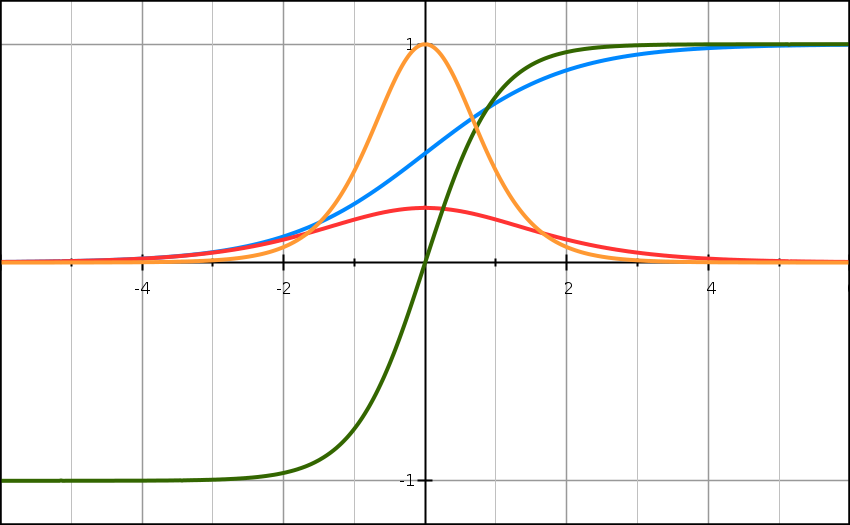
\includegraphics[width=.6\linewidth]{../results/q1_6_1.png}
    \caption{The plot of sigmoid function $\sigma(x)$ (in blue), its gradient $(1-\sigma(x))\sigma(x)$ (in red), the $\tanh(x)$ function (in green) and its gradient $1-\tanh^2(x)$ (in orange). }
    \label{fig:q1.6.1}
\end{figure}

\newpage

\subsection*{Q2.1.1}

If the weights and biases of every layer are initialized with zeros, the outpuut layer pre-activation values will be zeros regardless the input data and the post-activation values will be a uniform probability distribution.
In this case, there will still be gradients in the network due to the softmax loss, but they will be very small. Therefore the update of the network is very slow, the training process may terminate without convergence or the network may be stuck at local optima.
% Therefore The gradients of the network therefore will be zeros during training and the network weights will remain zeros after training.

\newpage

\subsection*{Q2.1.3}

Because if we initialize all the weights with the same number, some of them will have the same effect on the output values, and the gradients on them will be the same during backpropagation. Therefore, they will move together and hard to converge during training.

Because in one layer of neural net $\by=\bW\bx+\bb$, the variance of the output $\by$ depends on both the variance of input $\bx$ and variance of elements of the weight $\bW$ (output variance will be scaled by the number of input/output channels w.r.t the input variance). This is also true during the backpropagation of gradients. Therefore we scale the weight variance down by the layer size, To make the output variance of each layer equal to the input variance.

\newpage

\subsection*{Q3.1.2}

The progression of the loss and accuracy during different training processes is shown in Figure.~\ref{fig:q3.1.2}. Here the best learning rate I found is $2\times10^{-3}$.

Learning rates affect training process in the sense that the best learning rate gives the best convergence. Overly high or overly low learning rates will both slow down the convergence or make the training not able to converge to local optima.

Additionally, we can notice that large learning rates may cause the learning process to overshoot, which causes accuracy and loss to fluctuate during the training process.

The final test accuracy of the best network is $78\%$.

\begin{figure}[h!]
    \begin{subfigure}{.325\textwidth}
      \centering
      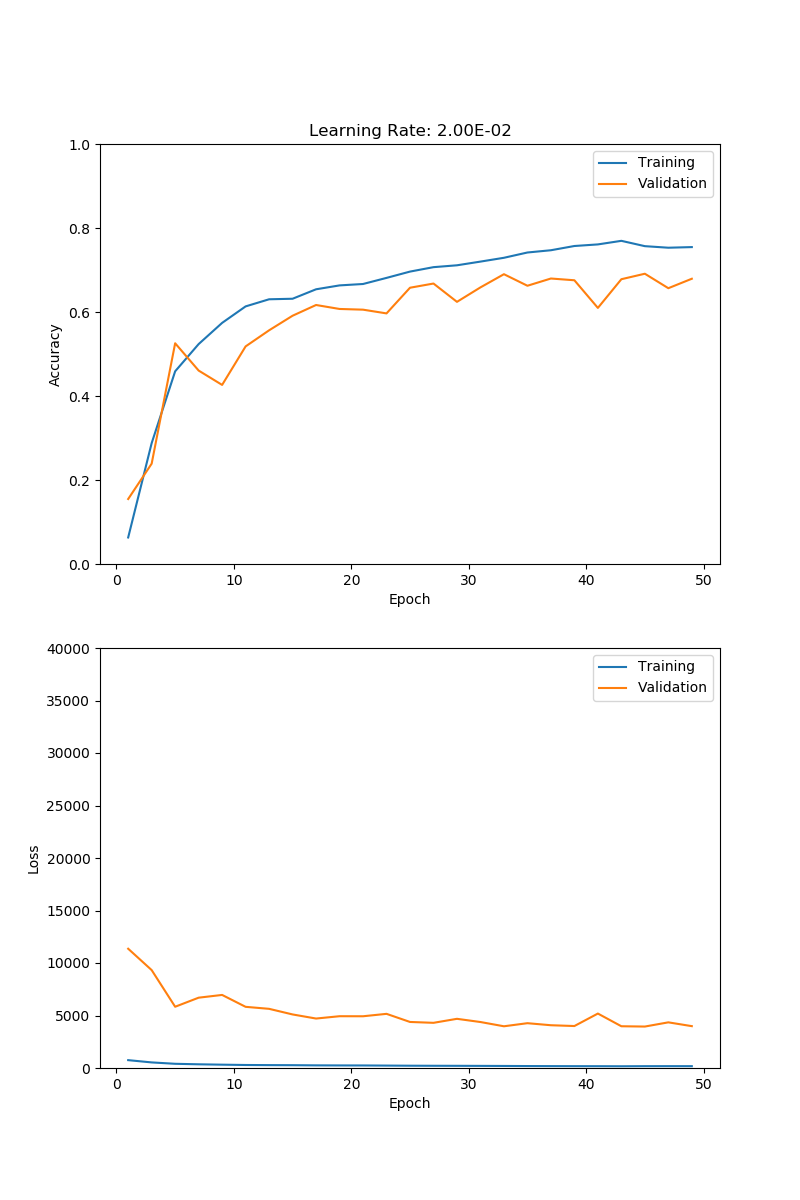
\includegraphics[width=.95\linewidth]{../results/q3_1_2_2E-02.png}
      \caption{Learning rate = $2\times10^{-2}$}
    \end{subfigure}
    \begin{subfigure}{.325\textwidth}
      \centering
      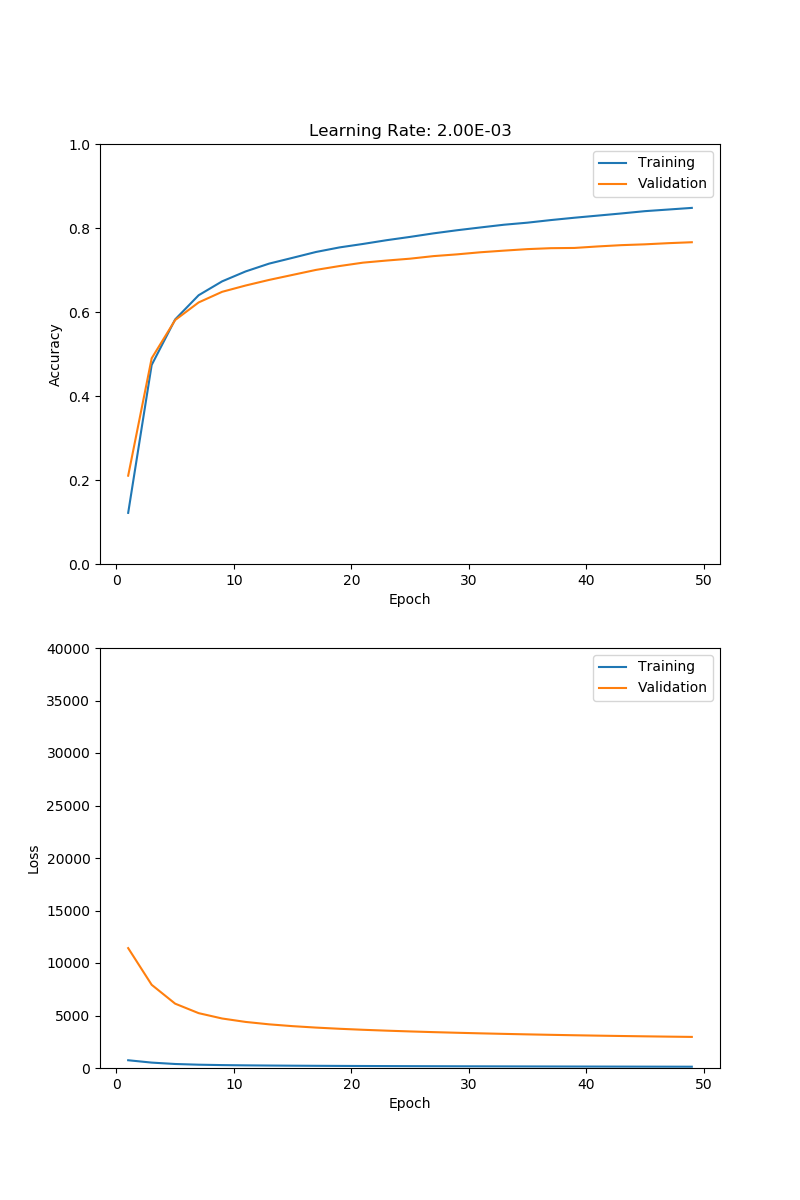
\includegraphics[width=.95\linewidth]{../results/q3_1_2_2E-03.png}
      \caption{Learning rate = $2\times10^{-3}$}
    \end{subfigure}
    \begin{subfigure}{.325\textwidth}
      \centering
      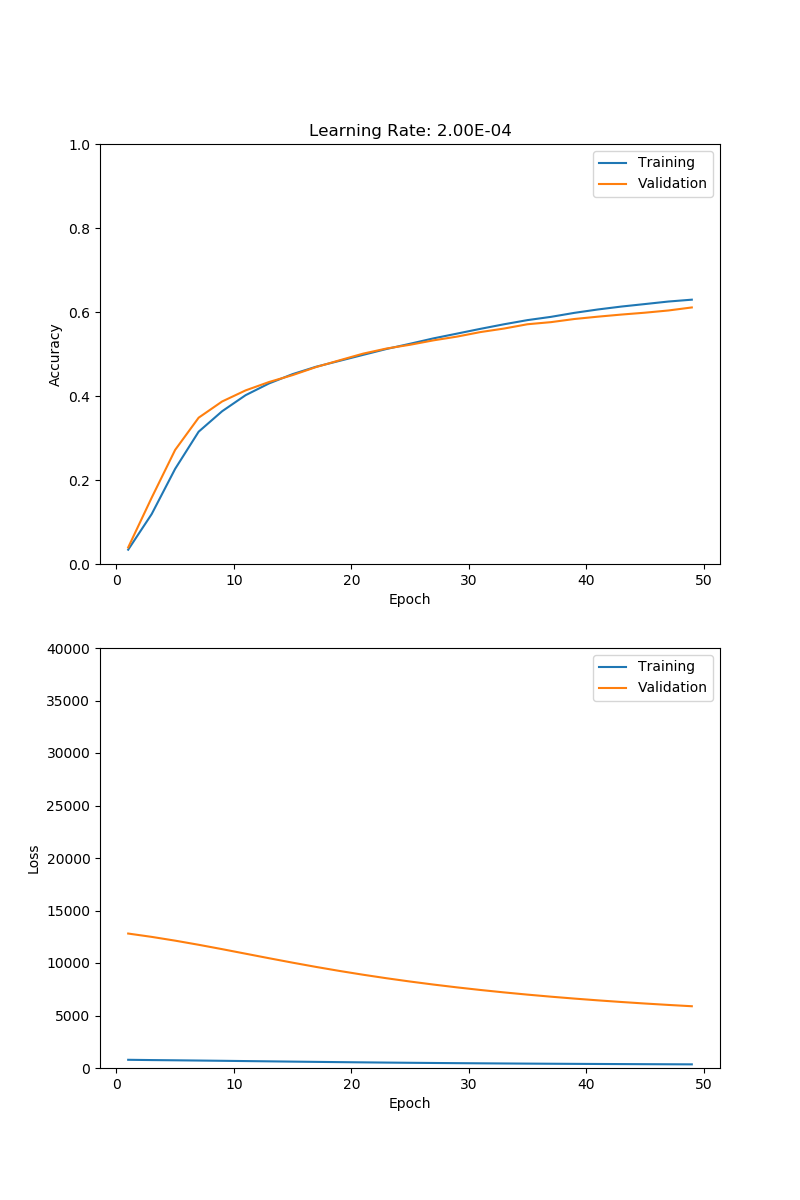
\includegraphics[width=.95\linewidth]{../results/q3_1_2_2E-04.png}
      \caption{Learning rate = $2\times10^{-4}$}
    \end{subfigure}\hfill
    \caption{Training progress on loss and accuracy using different learning rates. }
    \label{fig:q3.1.2}
\end{figure}

\newpage

\subsection*{Q3.1.3}

The weights of the first layer of the network is visualized in Figure.~\ref{fig:q3.1.3}. As we can observe, the weights after training is more structured and some of them resemble stroke curves of different digits and characters, and thus when we apply these weights, the input image that have similar strokes will have higher activation.

And before training, the visualized weights are just random noise and no structures or patterns can be observed.

\begin{figure}[h!]
    \begin{subfigure}{.495\textwidth}
      \centering
      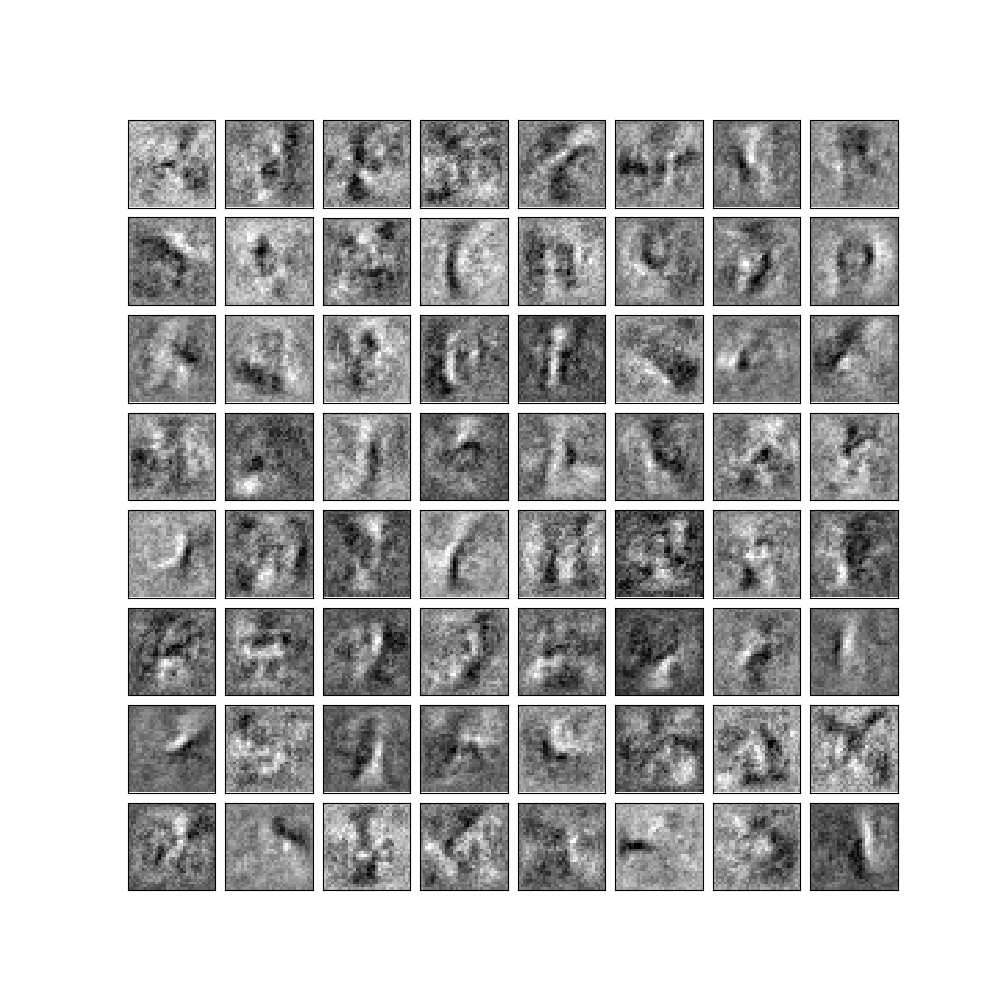
\includegraphics[width=.95\linewidth]{../results/q3_1_3a.png}
      \caption{After training}
    \end{subfigure}
    \begin{subfigure}{.495\textwidth}
      \centering
      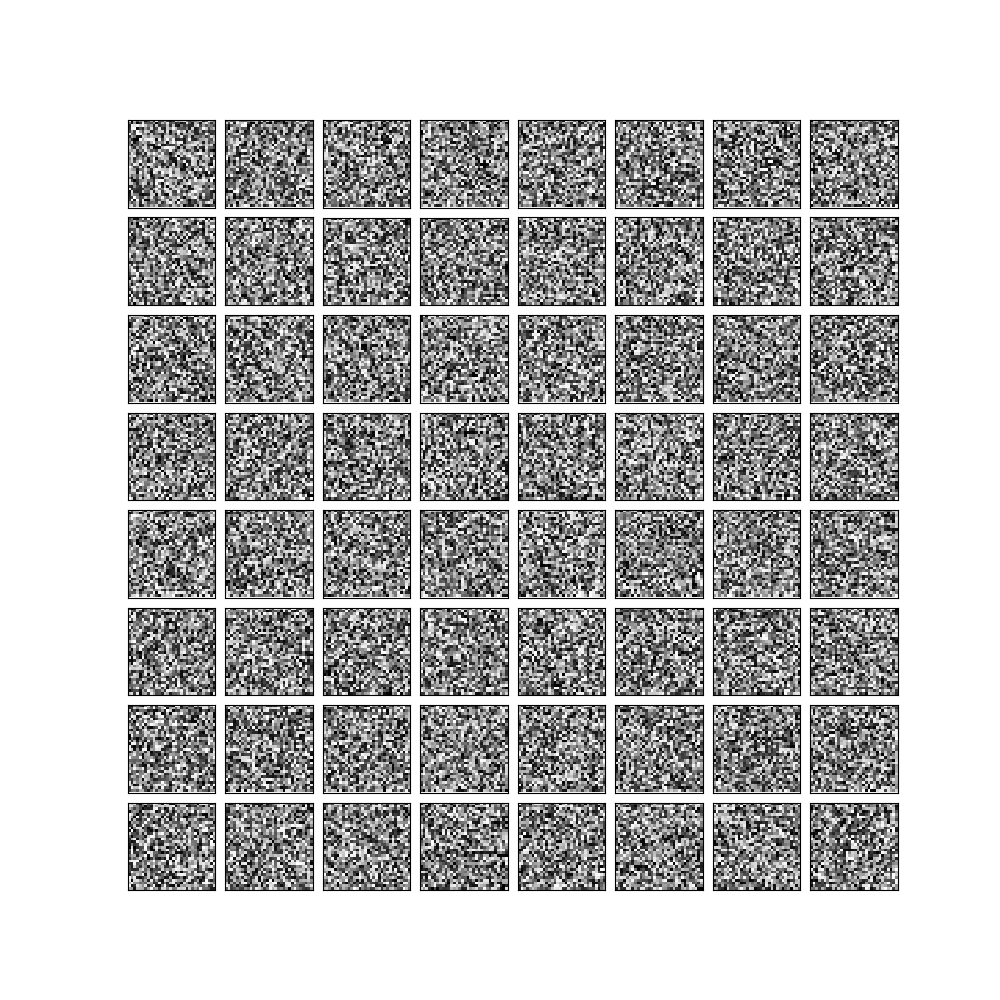
\includegraphics[width=.95\linewidth]{../results/q3_1_3b.png}
      \caption{Before training}
    \end{subfigure}\hfill
    \caption{Visualization of weights before and after training. }
    \label{fig:q3.1.3}
\end{figure}

\newpage

\subsection*{Q3.1.4}

The confusion matrix of the best model on the testing dataset is shown in Figure.~\ref{fig:q3.1.4}. As shown by some entries with high values in the matrix, the network is likely mix the digit ``0'' with the character `'O'', the character ``S'' with the digit ``5'', the character ``Z'' with the digit ``2'' and digit ``1'' with character ``I''. These results are quite reasonable as these pairs have very similar shape and even some human can get confused by them.

\begin{figure}[h!]
    \centering
    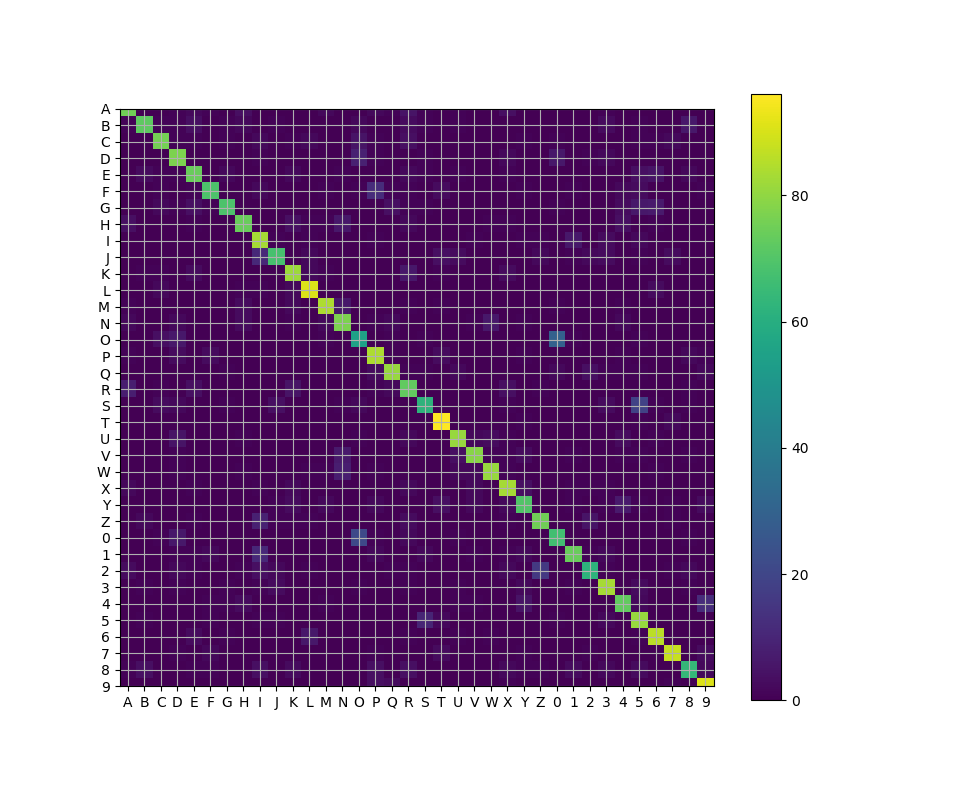
\includegraphics[width=.8\linewidth]{../results/q3_1_4.png}
    \caption{The confusion matrix of the best model on the testing dataset ($N=1800$). }
    \label{fig:q3.1.4}
\end{figure}

\newpage

\subsection*{Q4.1}

The first assumption made is that each character is connected within itself and well separate from others, although the morphological operations can help this to some extend. This means the method could fail if a character is splitted by background pixels or is connected to others by foreground pixels. Some examples where the method could fail are shown in Figure.~\ref{fig:q4.1} (a).

The second assumption is that all character are written in the upright form (no large rotation is applied), each line of text is written horizontallly and text is written line by line. The method could fail if the text are written with large rotation, as shown in Figure.~\ref{fig:q4.1} (b).

\begin{figure}[h!]
    \begin{subfigure}{.495\textwidth}
      \centering
      
\includegraphics[width=.5\linewidth]{../results/q4_1a.png}
      \caption{The characters that are connected to each other (``ABC'') or divided into multiple parts (``D''). }
    \end{subfigure}
    \begin{subfigure}{.495\textwidth}
      \centering
      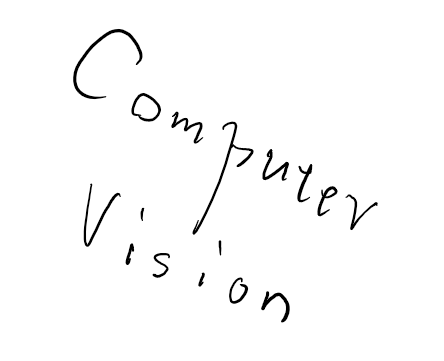
\includegraphics[width=.5\linewidth]{../results/q4_1b.png}
      \caption{The characters that are not written in horizontal and rotated. }
    \end{subfigure}\hfill
    \caption{Possible failure cases of the text extraction pipeline. }
    \label{fig:q4.1}
\end{figure}

\newpage

\subsection*{Q4.3}

The character detection results are shown in Figure.~\ref{fig:q4.3}. Note that the bounding boxes are directly estimate from the connected pixels and thus they are not padded by now. And we can see that all characters and digits are successfully detected and located, which means the accuracy of \code{findLetters(..)} is $100\%$.

\begin{figure}[h!]
    \begin{subfigure}{.495\textwidth}
      \centering
      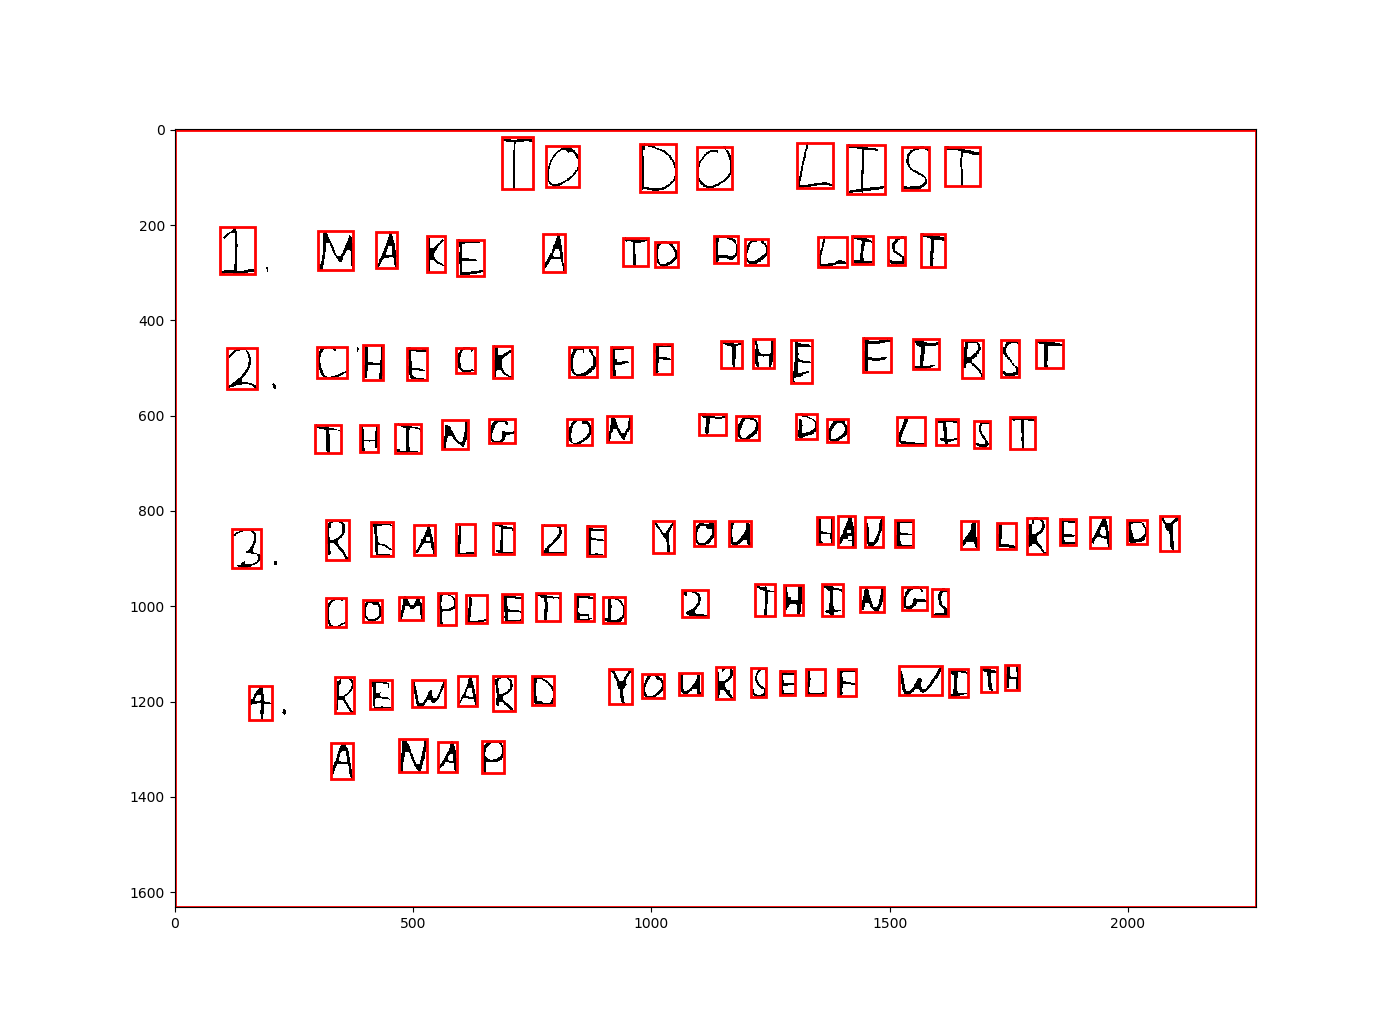
\includegraphics[width=.9\linewidth]{../results/q4_3_1.png}
      \caption{The detection result of the first image. }
    \end{subfigure}
    \begin{subfigure}{.495\textwidth}
      \centering
      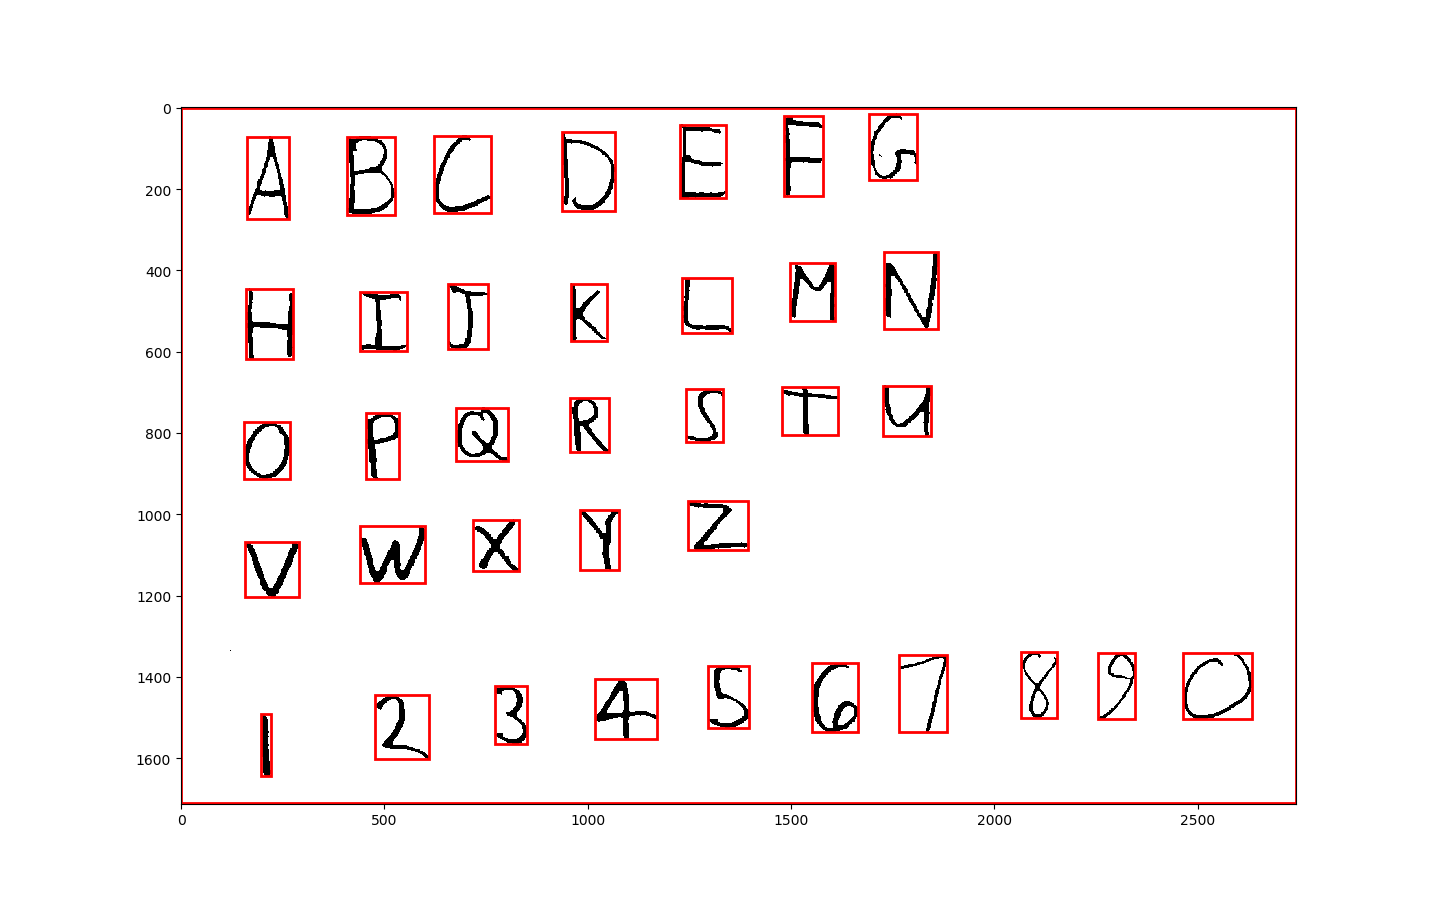
\includegraphics[width=.9\linewidth]{../results/q4_3_2.png}
      \caption{The detection result of the second image. }
    \end{subfigure}\hfill
    \begin{subfigure}{.495\textwidth}
      \centering
      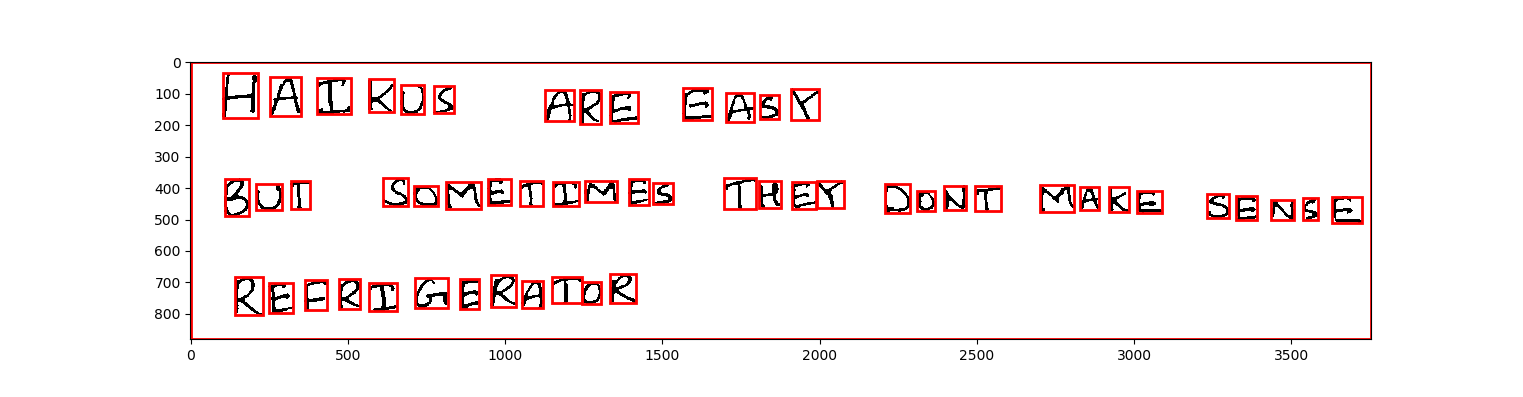
\includegraphics[width=.9\linewidth]{../results/q4_3_3.png}
      \caption{The detection result of the third image. }
    \end{subfigure}
    \begin{subfigure}{.495\textwidth}
      \centering
      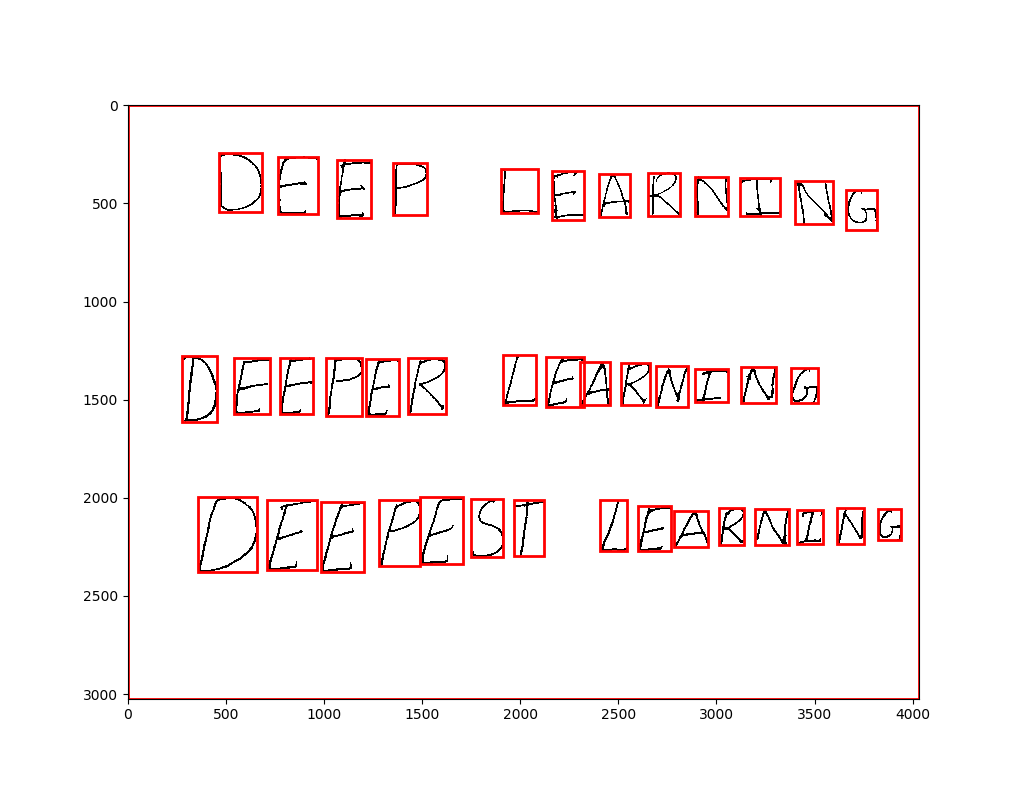
\includegraphics[width=.9\linewidth]{../results/q4_3_4.png}
      \caption{The detection result of the fourth image. }
    \end{subfigure}\hfill
    \caption{Detection results of characters in images in bounding boxes. }
    \label{fig:q4.3}
\end{figure}

\newpage
\subsection*{Q4.4}

The extracted texts from each image and their accuracies are shown as follows:

\begin{verbatim}
Image: 01_list.jpg
T0D0LI5T
IMAKEAT0DOLIST
2CHFCK0FETHIFIRST
THING0NT0O0LIST
3RIALIZEY0UHAVEALR2ADT
C0MPL5T5D2THINGS
4XXWARDY0URSELFWITH
ANAP
Accuracy: 0.800

Image: 02_letters.jpg
XBCDEFG
HITKLMN
0PQRSTU
VWXYZ
1X3GS67X90
Accuracy: 0.806

Image: 03_haiku.jpg
HAIKUSAREEASY
EUTSQMETIMESTREYD0NTMAK2SENQE
REFRIGERAT0R
Accuracy: 0.852

Image: 04_deep.jpg
DEEPLEARMING
CEEPTRLEARNING
5EEAE5TIEARNING
Accuracy: 0.829
\end{verbatim}

\newpage

\subsection*{Q5.2}

The plotted training loss is shown in Figure.~\ref{fig:q5.2}.

As training process progresses, the training loss first drops quickly and then plateau at the low level. The overall training loss curve is very smooth.
This shows the momentum used in gradient descent can help speed up the loss reduction process.

\begin{figure}[h!]
    \centering
    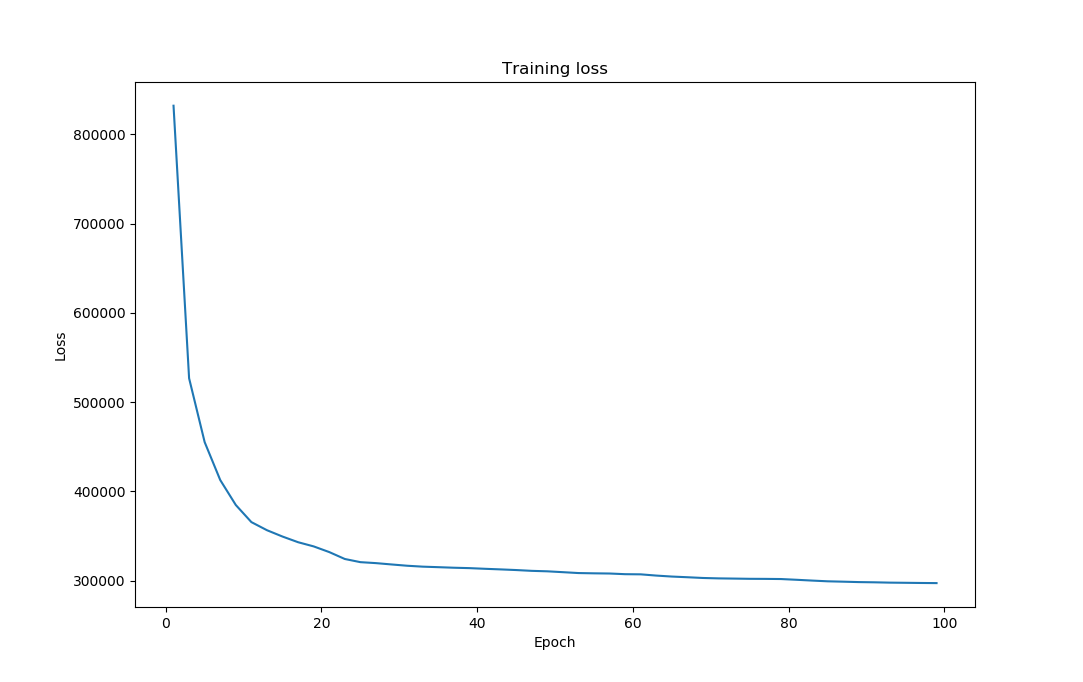
\includegraphics[width=.8\linewidth]{../results/q5_2.png}
    \caption{The training loss curve of the Autoencoder. }
    \label{fig:q5.2}
\end{figure}

\newpage

\subsection*{Q5.3.1}

The validation images and their reconstructions results are shown in Figure.~\ref{fig:q5.3.1}. As shown in the figure, the reconstructions results is more blur compared to the input images. Moreover, there is circle ``area of reconstruction'', and the contents within that circle can be better reconstructed than those outside (As shown by the first row of Figure.~\ref{fig:q5.3.1}). This is probably because the contents of training images are mostly centered in that circle.

\begin{figure}[h!]
    \centering
    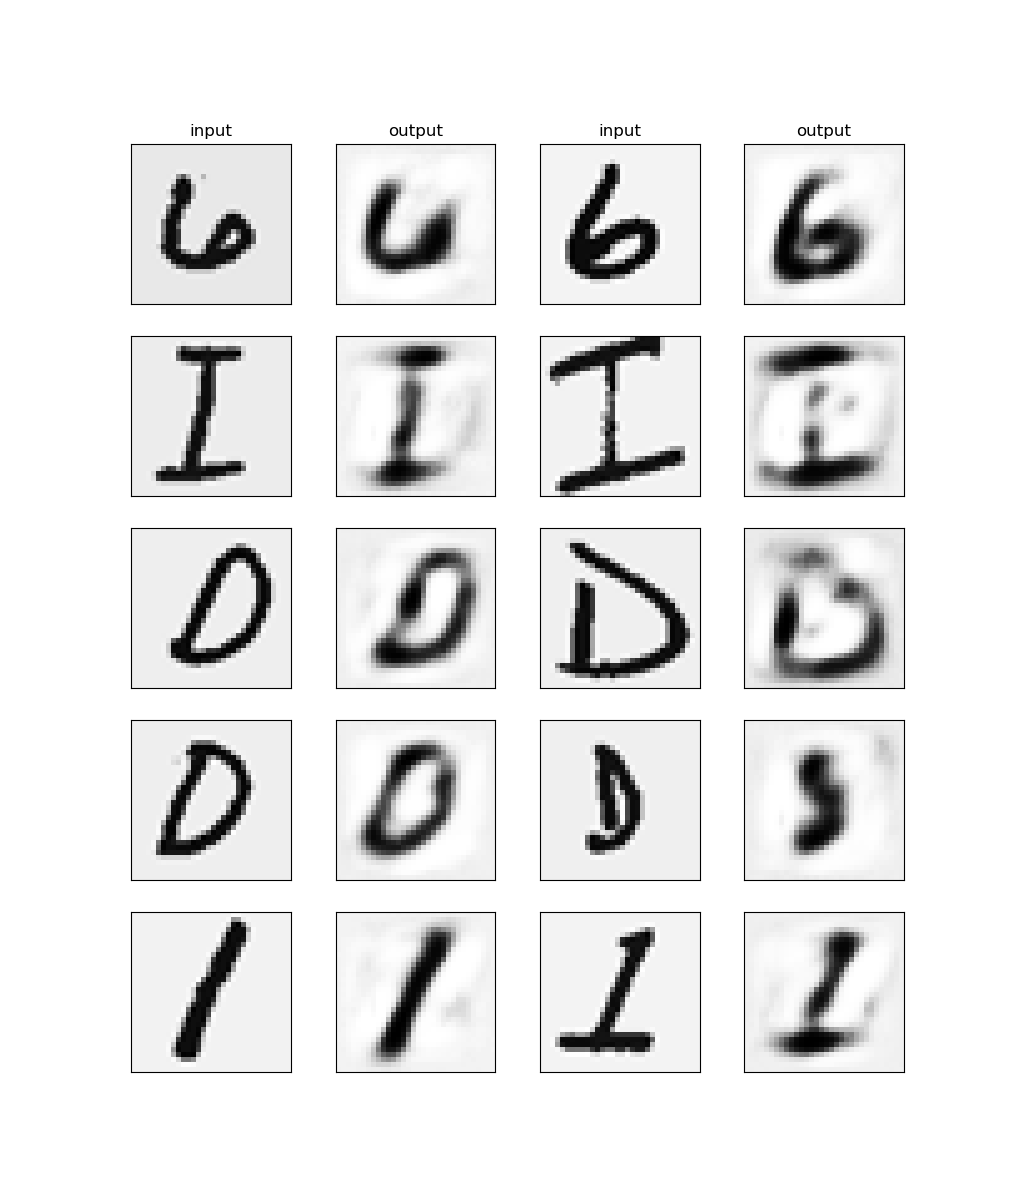
\includegraphics[width=.8\linewidth]{../results/q5_3_1.png}
    \caption{The validation images (input) and their reconstructions (output) using Autoencoder. }
    \label{fig:q5.3.1}
\end{figure}

\newpage

\subsection*{Q5.3.2}

The average PSNR over the validation set is 16.085.

\newpage

\subsection*{Q6.1}

\newcommand{\bX}{\mathbf{X}}
\newcommand{\bA}{\mathbf{A}}
\newcommand{\bC}{\mathbf{C}}
\newcommand{\bU}{\mathbf{U}}
\newcommand{\bu}{\mathbf{u}}
\newcommand{\bV}{\mathbf{V}}
\newcommand{\bv}{\mathbf{v}}
\newcommand{\bS}{\mathbf{S}}
\newcommand{\bP}{\mathbf{P}}

\textbf{Note} in this theory question, I treat the dimension of the data matrix to be (number of features, number of datapoints), and thus during the whole deduction, the dimension is the transpose of default setting in implementation.
% The final dimension of the projection matrix should be the same ($32\times1024$) but will differ in terms of left- or right-multiply.

Suppose our data matrix is $\bA \in \mathbb{R}^{M\times N}$, where $N$ is the number of data points in the dataset and $M$ is number of dimension for each data point (here is the number of pixels in each image). Then each column of $\bX$ is a datapoint, and consider the SVD decomposition
\begin{align} \label{eq:SVD}
  \bA = \bU\bS\bV^T  = \sum_{i=1}^K \bu_i \sigma_i \bv_i^T,
\end{align}
where $K=\min\{M, N\}$, $\bu_i$, $\bv_i$ is the $i^{th}$ column of $\bU$ and $\bV$ respectively,
and $\sigma_i$ is the $i^{th}$ diagonal element in $\bS$.

To give the best $k$-rank approximation of $\bA$ in terms of frobenius, we can simply take the first $k$ terms in the summation in Eq.~\ref{eq:SVD}, which means
\begin{align}
  \hat{\bA} = \sum_{i=1}^k \bu_i \sigma_i \bv_i^T = \bX \bC,
\end{align}
where the principle components $\bX$ and the compressed data matrix $\bC$ are defined to be
\begin{align}
  \bX = [ \bu_1\;\bu_2\;\dots\;\bu_k ] \quad
  \bC =
  \begin{bmatrix}
    \sigma_1\bv_1^T \\ \sigma_2\bv_2^T \\ \dots \\ \sigma_k\bv_k^T
  \end{bmatrix},
\end{align}
where each column of $\bC$ is a compressed representation of the original data point in the corresponding column of $\bA$.

To get $\bC$ for any other input $\bA'$, we can simply simply calculate $\bX^T\bA'$, where we can define $\bP = \bX^T$ as the projection matrix
In our case, $M=1024$ and $k=32$, and thus the size of the projection matrix $\bP$ is $(32 \times 1024)$ and its rank is 32.

\textbf{Note}: In the case where the first dimension is the number of datapoint (as in our implementation), the shape of the projection matrix will be $(1024 \times 32)$ and needs to be right-multiplied to the input data matrix.

\newpage

\subsection*{Q6.2}

The validation images and their reconstructions results using PCA are shown in Figure.~\ref{fig:q5.3.1}. As we can see, besides that the output are blur, the reconstructed images are generally more gray.

The average PSNR over the validation set is 16.347, which is higher than that obtained from Autoencoder, and means better reconstruction quality.

\begin{figure}[h!]
    \centering
    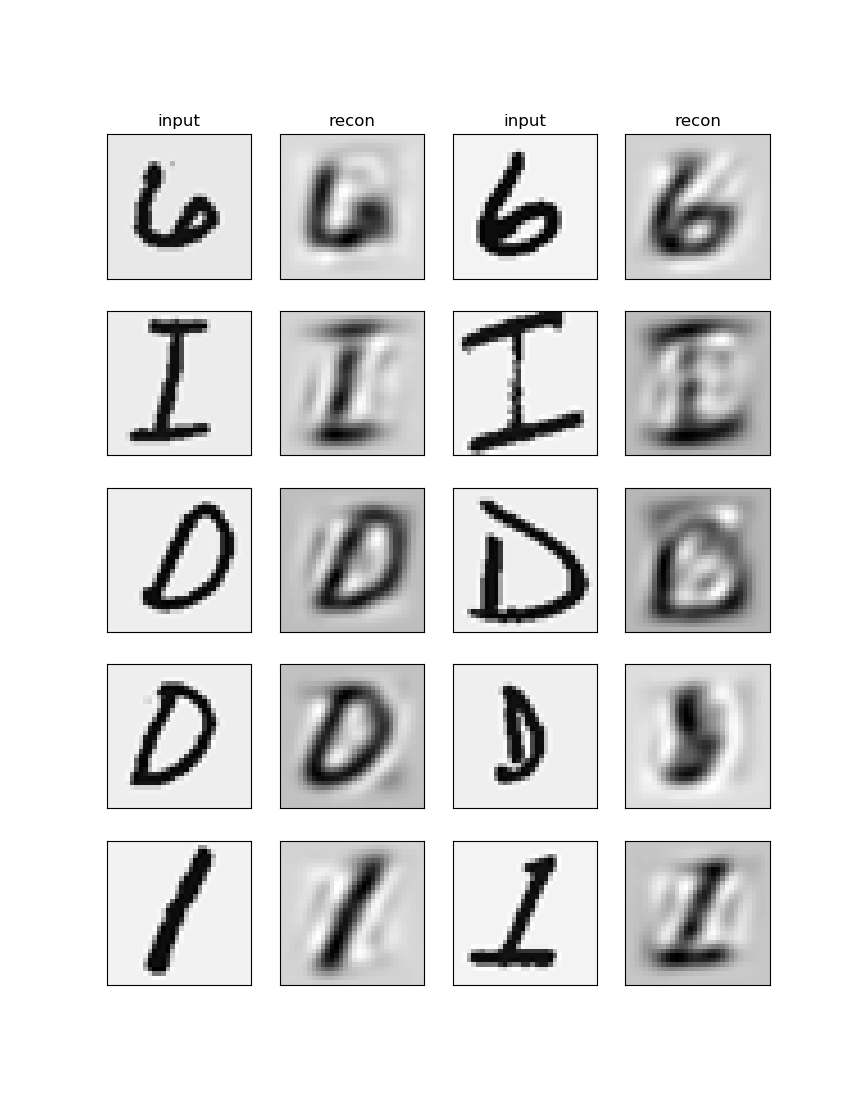
\includegraphics[width=.8\linewidth]{../results/q6_2.png}
    \caption{The validation images (input) and their reconstructions (recon) using PCA. }
    \label{fig:q6.2}
\end{figure}

\newpage
\subsection*{Q7.1.1}

For this question, please run \code{python run\_q7\_1.py 7.1.1}.

The loss and accuracy during the training process is show in Figure.~\ref{fig:q7.1.1}

\begin{figure}[h!]
    \centering
    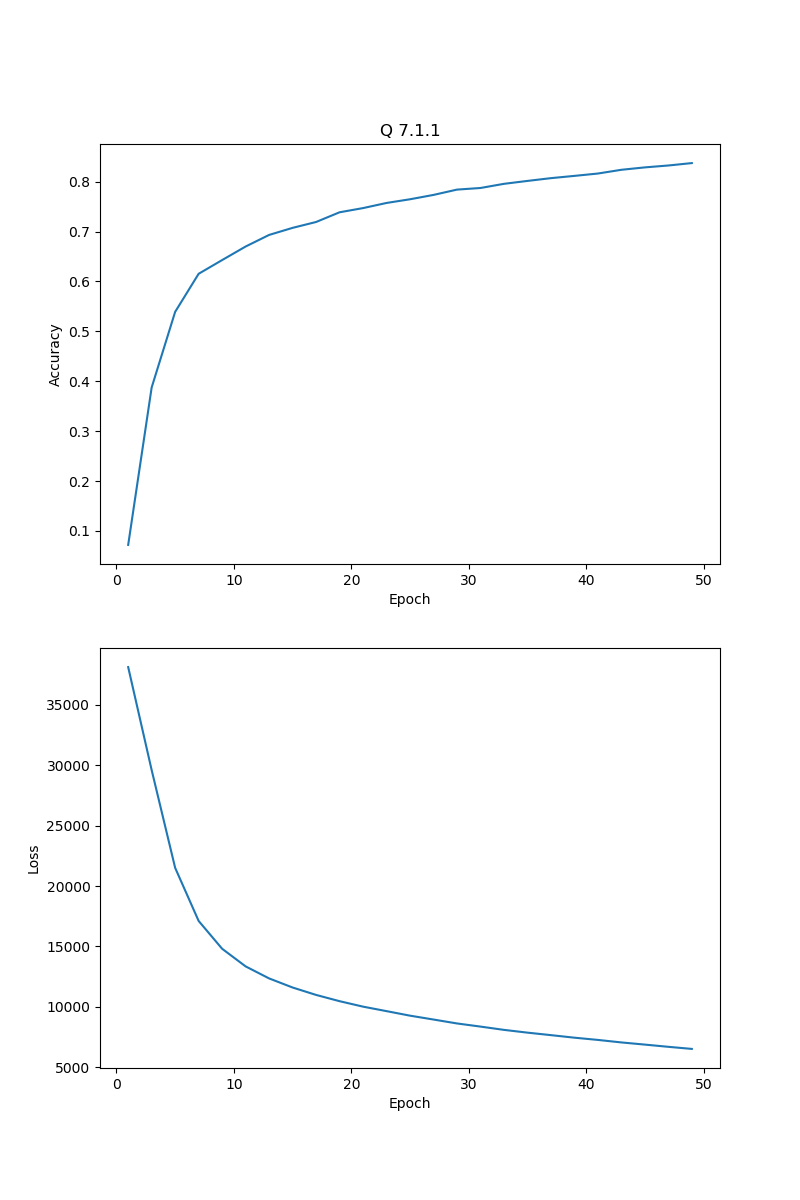
\includegraphics[width=.6\linewidth]{../results/q7_1_1.png}
    \caption{The training progress of the fully-connected network on NIST36 dataset. }
    \label{fig:q7.1.1}
\end{figure}

\newpage
\subsection*{Q7.1.2}

For this question, please run \code{python run\_q7\_1.py 7.1.2}.

The loss and accuracy during the training process is show in Figure.~\ref{fig:q7.1.2}

\begin{figure}[h!]
    \centering
    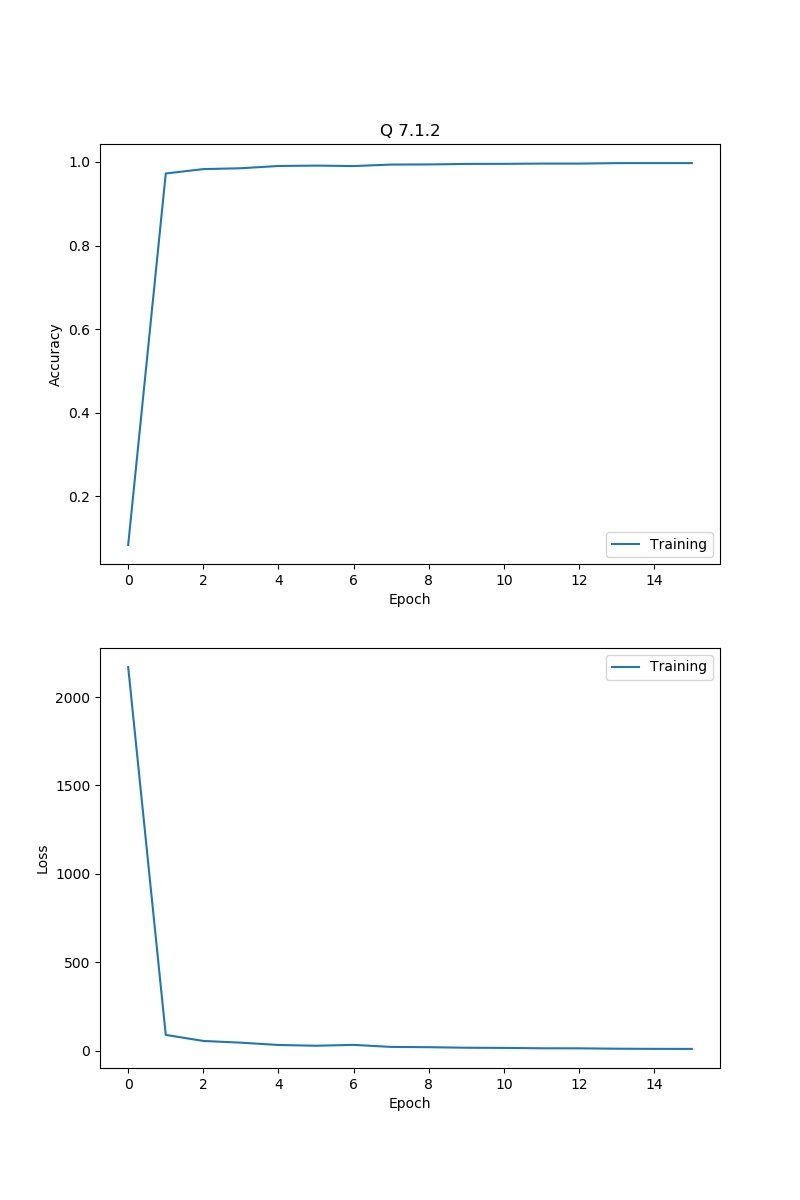
\includegraphics[width=.6\linewidth]{../results/q7_1_2.png}
    \caption{The training progress of a CNN on MNIST dataset. }
    \label{fig:q7.1.2}
\end{figure}

\newpage
\subsection*{Q7.1.3}

For this question, please run \code{python run\_q7\_1.py 7.1.3}.

The loss and accuracy during the training process is show in Figure.~\ref{fig:q7.1.3}

\begin{figure}[h!]
    \centering
    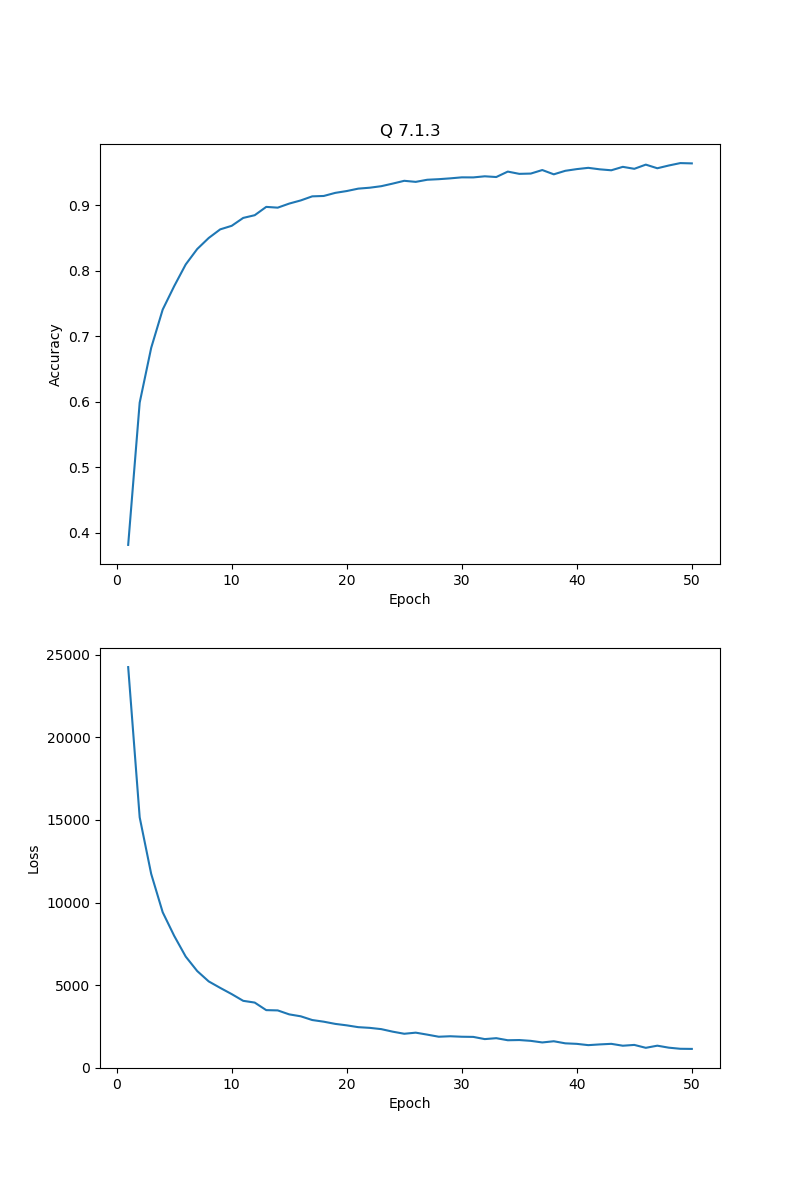
\includegraphics[width=.6\linewidth]{../results/q7_1_3.png}
    \caption{The training progress of a CNN on NIST36 dataset. }
    \label{fig:q7.1.3}
\end{figure}

\newpage
\subsection*{Q7.1.4}

For this question, please run \code{python run\_q7\_1.py 7.1.4 train} to train the CNN on EMNIST Balanced dataset and \code{python run\_q7\_1.py 7.1.4 test} to test the trained CNN on the texts detected and cropped from the given 4 images.

The loss and accuracy during the training process is show in Figure.~\ref{fig:q7.1.4}. The test results and accuracy on the text given by findLetters is shown as follows:

\begin{figure}[h!]
    \centering
    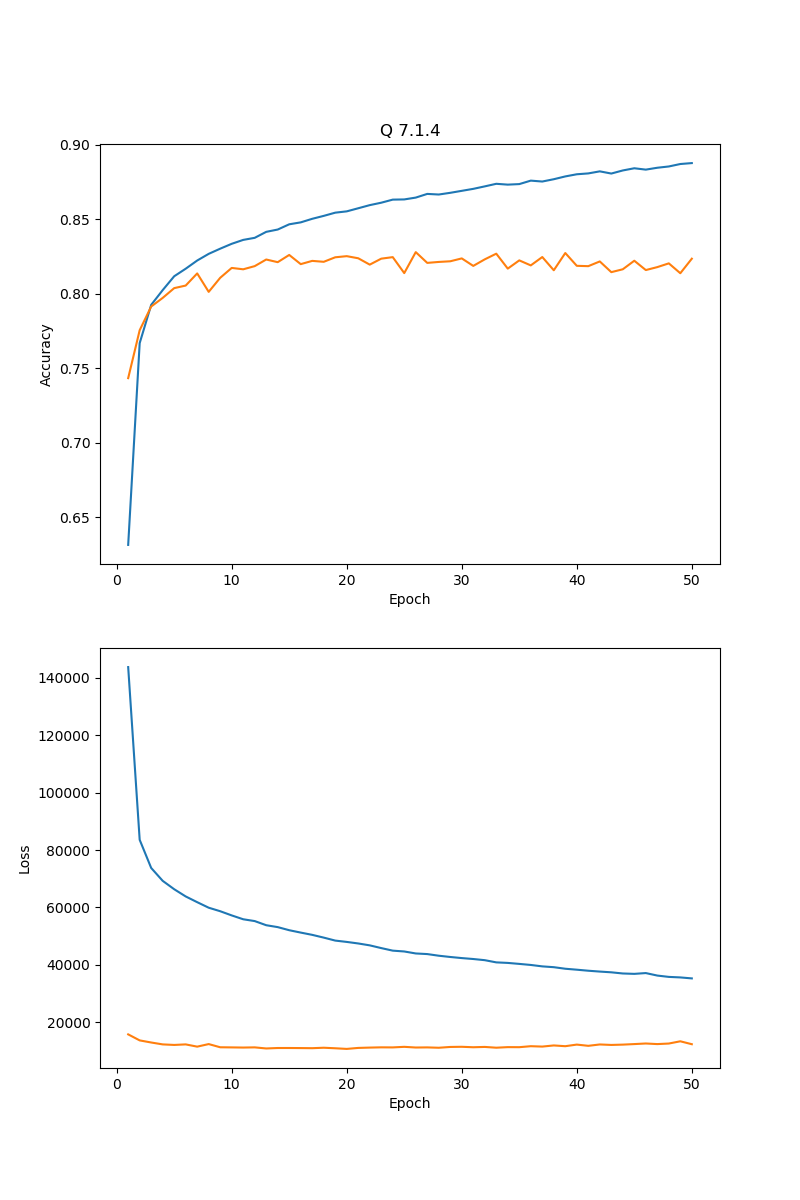
\includegraphics[width=.6\linewidth]{../results/q7_1_4.png}
    \caption{The training progress of a CNN on EMNIST Balanced dataset. }
    \label{fig:q7.1.4}
\end{figure}

\begin{verbatim}
  Image: 01_list.jpg
  T0D0LZST
  IMgXEAT0B0LISF
  2CHECK0FFTHEFERST
  THINGQNT0DgLE5T
  3REALI2EY0UHBVEgLREADY
  C0MPLETED2THEWGS
  gREWARDY0WRSELFWITH
  ANgP
  Accuracy: 0.757

  Image: 02_letters.jpg
  gBCDEFG
  HIJKLMN
  0PQRSTU
  VWXYZ
  I23q5G78gC
  Accuracy: 0.806

  Image: 03_haiku.jpg
  HAIKUSAREEAgY
  BUFS0METqMEgTHEYDaNTMAKESEMgE
  REfRgGERQT0R
  Accuracy: 0.759

  Image: 04_deep.jpg
  DEEPLEARnIHG
  BEEPERLEARNING
  DEEPESJZEgRQING
  Accuracy: 0.829
\end{verbatim}

\newpage
\subsection*{Q7.2.1}

Please use one of the following lines of script to run the experiment using SqueezeNet or a small CNN on Oxford flowers 17 or flowers 102 dataset.

\begin{verbatim}
  python run_q7_2.py 17 small
  python run_q7_2.py 102 small
  python run_q7_2.py 17 squeeze
  python run_q7_2.py 102 squeeze
\end{verbatim}

In this question, I designed a small CNN containing 3 convolution layers with ReLU activation, and dropout layers, followed by two-layer fully connected network.
The training progress of above experiment are shown in Figure.~\ref{fig:q7.2.1} and Figure.~\ref{fig:q7.2.2}.
As we can see from those figures, the network based on pretrained SqueezeNet yeild faster training progress and better training results than the small CNN trained from scratch.
Moreover, interestingly, during finetuning the SqueezeNet, we can notice a slowdown around epoch 5.
% This is probably because at first, the pretrained network contains bias and it takes some time to overcome them and reach a general distribution.

\begin{figure}[h!]
    \begin{subfigure}{.495\textwidth}
      \centering
      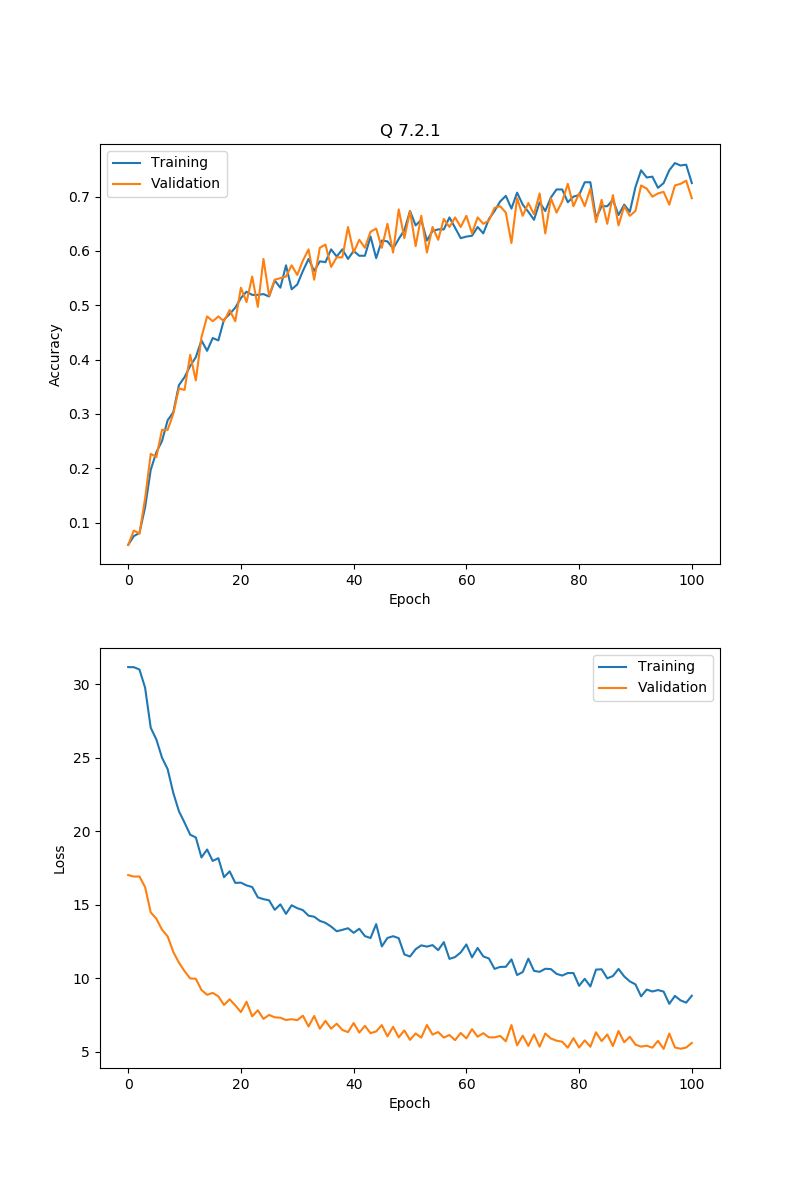
\includegraphics[width=.9\linewidth]{../results/q7_2_1_17_small.png}
      \caption{Using a small CNN. }
    \end{subfigure}
    \begin{subfigure}{.495\textwidth}
      \centering
      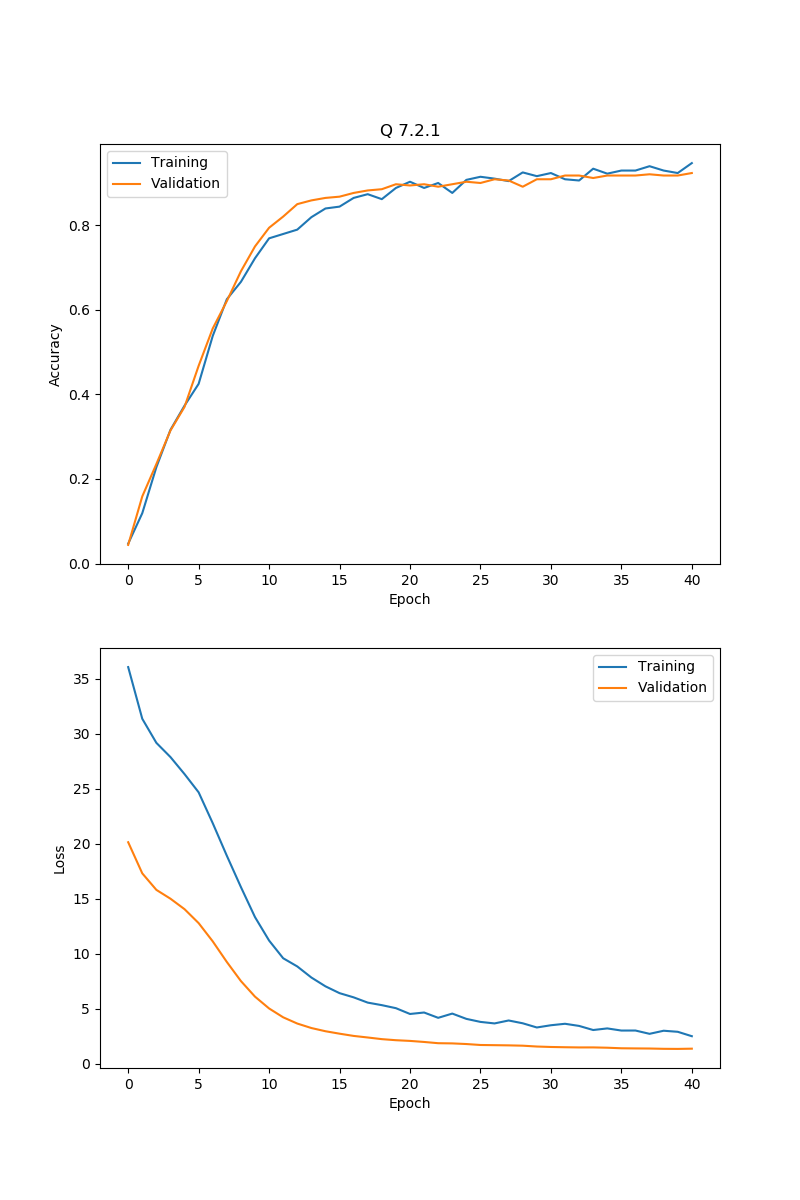
\includegraphics[width=.9\linewidth]{../results/q7_2_1_17_squeeze.png}
      \caption{Using pretrained SqueezeNet. }
    \end{subfigure}\hfill
    \caption{Training progress on Oxford flower 17 dataset. }
    \label{fig:q7.2.1}
\end{figure}

\begin{figure}[h!]
    \begin{subfigure}{.495\textwidth}
      \centering
      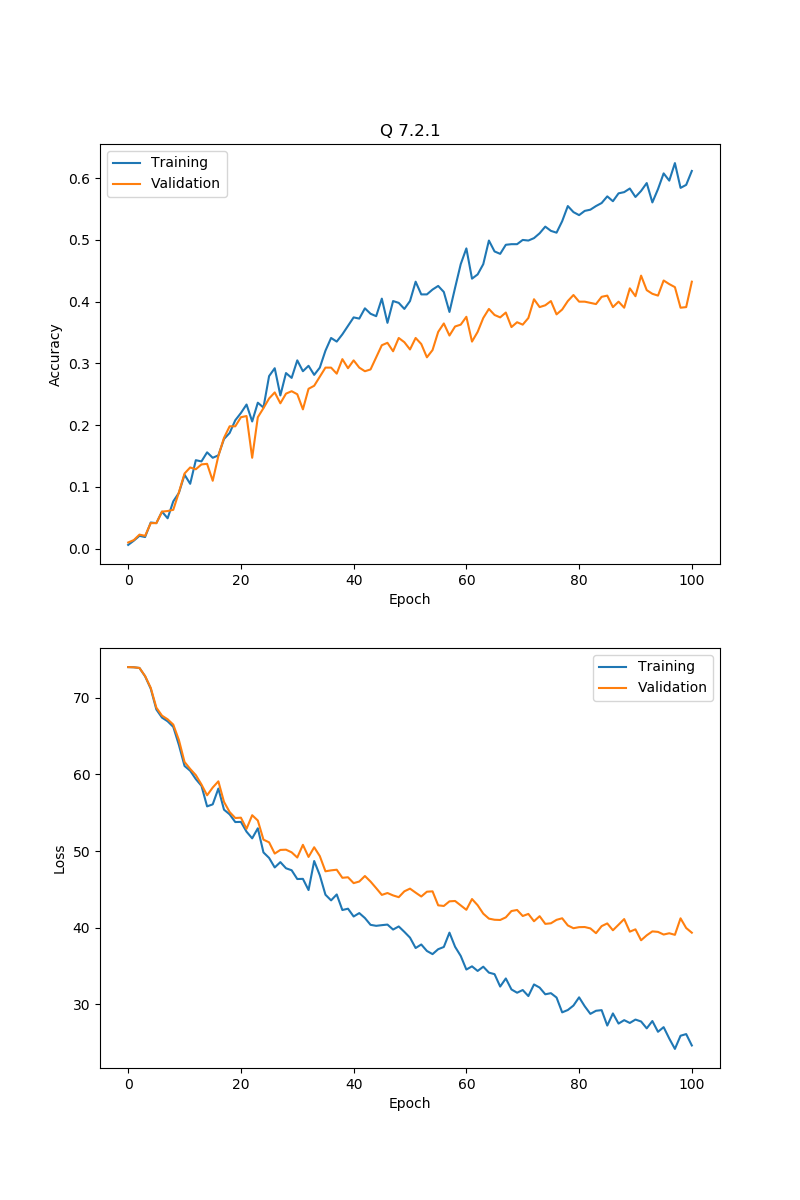
\includegraphics[width=.9\linewidth]{../results/q7_2_1_102_small.png}
      \caption{Using a small CNN. }
    \end{subfigure}
    \begin{subfigure}{.495\textwidth}
      \centering
      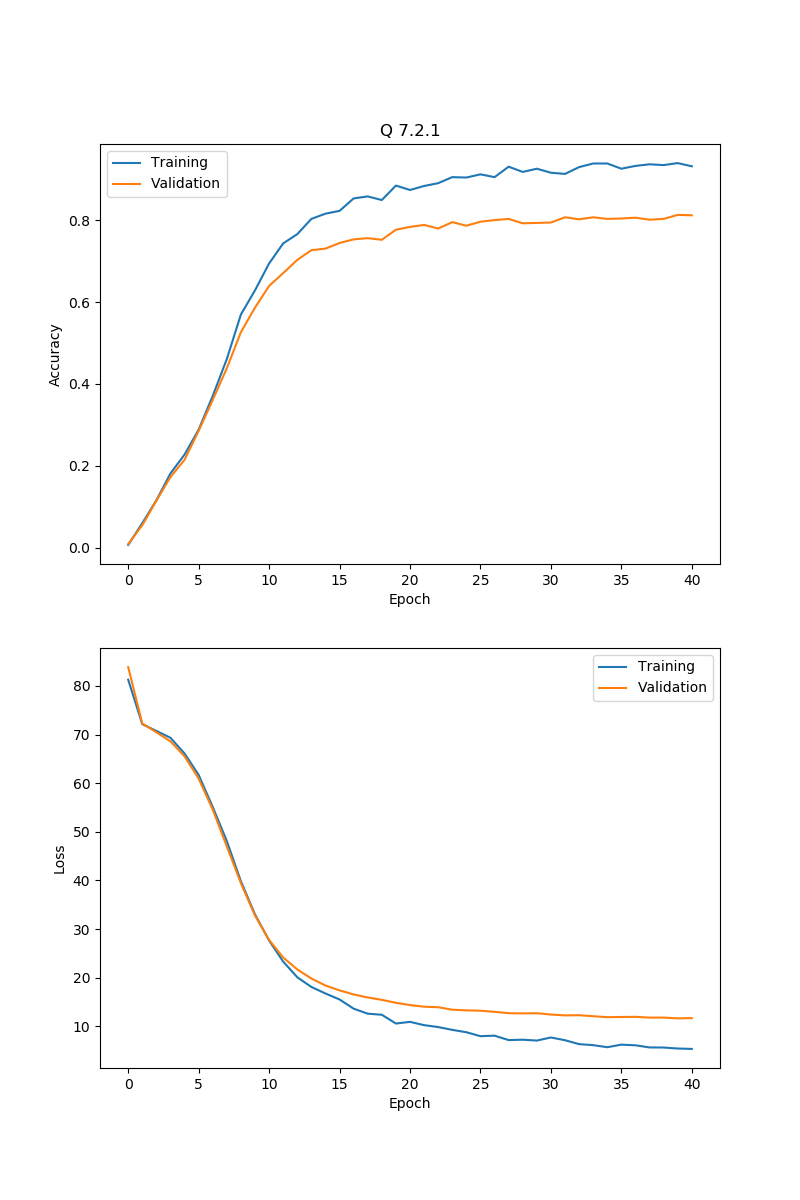
\includegraphics[width=.9\linewidth]{../results/q7_2_1_102_squeeze.png}
      \caption{Using pretrained SqueezeNet. }
    \end{subfigure}\hfill
    \caption{Training progress on Oxford flower 102 dataset. }
    \label{fig:q7.2.2}
\end{figure}


\end{document}
